\chapter{Introduction}
The traditional approach to Agent-Based Simulation (ABS) has so far always been object-oriented techniques, due to the influence of the seminal work of Epstein et al \cite{epstein_growing_1996} in which the authors claim "[..] object-oriented programming to be a particularly natural development environment for Sugarscape specifically and artificial societies generally [..]" (p. 179). This work established the metaphor in the ABS community, that \textit{agents map naturally to objects} \cite{north_managing_2007} which still holds up today.

This thesis challenges that metaphor and explores ways of approaching ABS with the functional programming paradigm using the language Haskell. It is the first one to do so on a \textit{systematical} level and develops a foundation by presenting fundamental concepts and advanced features to show how to leverage the benefits of it \cite{hudak_haskell_1994, hudak_history_2007} to become available when implementing ABS functionally. By doing this, the thesis both shows \textit{how} to implement ABS purely functional and \textit{why} it is of benefit of doing so, what the drawbacks are and also when a pure functional approach should \textit{not} be used. 

This thesis claims that the agent-based simulation community needs functional programming because of its \textit{scientific computing} nature where results need to be reproducible and correct while simulations should be able to massively scale-up as well. The established object-oriented approaches need considerably high effort and might even fail to deliver these objectives due to its conceptually different approach to computing. In contrast, this thesis will show that by using functional programming for implementing ABS it is easy to add parallelism and concurrency, the resulting simulations are easy to test and verify, suitable to apply new testing methods like property-based testing, guaranteed to be reproducible already at compile-time, have fewer potential sources of bugs and thus can raise the level of confidence in the correctness of an implementation to a new level.

--------------

This chapter is the introduction to the thesis ("why do we need functional programming in ABS?") and motivates it and describes the aim and scope of the Ph.D. Further it states the hypotheses and contributions. 
\begin{itemize}
	\item Main Argument: Defining the problem, motivation, aim and scope of the Ph.D.
	\item Hypotheses: Precisely stating the hypotheses which will form the points of reference for the whole research.
	\item Contributions: Precisely list the contribution to knowledge this Ph.D. makes and list all papers which were written (and published) during this Ph.D.
\end{itemize}

TODO: understand Gintis failure (read gintis paper and the masterthesis)

Argument \& Story of my Thesis with the components (publications) i have so far and which i still plan to do

dependent types will be put to rest unless there is really some time left (which i doubt) and will be considered in the final thesis but only on a conceptual level without going into lot of technical detail because: 1. i didn't do enough research on it and 2. dependent types seem to be nearly out of focus of the thesis. Dependent Types sections will be written very late, after the finished research has been incorporated, and if at that point i have come to the conclusion that it is too unfinished / vague / not substantial enough then i will simply skip this part (or if it is too long already and the contribution is enough already withouth dependent types).

\section{Publications}
Throughout the course of the Ph.D. four (4) papers were published:

\begin{enumerate}
	\item The Art Of Iterating - Update Strategies in Agent-Based Simulation \cite{thaler_art_2017} - This paper derives the 4 different update-strategies and their properties possible in time-driven ABS and discusses them from a programming-paradigm agnostic point of view. It is the first paper which makes the very basics of update-semantics clear on a conceptual level and is necessary to understand the options one has when implementing time-driven ABS purely functional.
	
	\item Pure Functional Epidemics \cite{thaler_pure_2019} - This paper establishes in technical detail \textit{how} to implement ABS in Haskell using non-monadic FRP with Yampa and monadic FRP with Dunai. It outlines benefits and drawbacks and also touches on important points which were out of scope and lack of space in this paper but which will be addressed in the Methodology chapter of this thesis.
	
	\item A Tale Of Lock-Free Agents (TODO cite) - This paper is the first to discuss the use of Software Transactional Memory (STM) for implementing concurrent ABS both on a conceptual and on a technical level. It presents two case-studies, with the agent-based SIR model as the first and the famous SugarScape being the second one. In both case-studies it compares performance of STM and lock-based implementations in Haskell and object-oriented implementations of established languages. Although STM is now not unique to Haskell any more, this paper shows why Haskell is particularly well suited for the use of STM and is the only language which can overcome the central problem of how to prevent persistent side-effects in retry-semantics. It does not go into technical details of functional programming as it is written for a simulation Journal.

	\item Hands Off My Property (TODO cite) - This paper is the first to apply property-based testing, as in Haskells QuickCheck and SmallCheck libraries, to test and verify ABS implementations. It discusses the problem mainly on a conceptual level without going too much into detail as it is targeted towards a simulation Journal / Conference. Also it argues that by simply using Haskell as implementation language one gets automatically rid of a large class of run-time bugs which can occur in the established languages. Further it shows that the use of Haskell makes it easier to test and verify ABS because code tends to be more modular and thus easier tested and reasoned about, which is particularly well supported in Haskell due to the strong static type system and explicitness / lack of side-effects.
\end{enumerate}

There has been unpublished work as well:

\begin{enumerate}
	\item Towards Pure Functional Agent-Based Simulation (TODO cite) - This paper summarizes the main benefits of using pure functional programming as in Haskell to implement ABS and discusses on a conceptual level how to implement it and also what potential drawbacks are and where the use of a functional approach is not encouraged. It is written as a conceptual / review paper, which tries to "sell" pure functional programming to the agent-based community without too much technical detail and parlance where it refers to the important technical literature from where an interested reader can start.

% only if really finished / submitted
	\item The Equilibrium - Totality Correspondence (TODO cite) - This extended abstract is the first which conceptually investigates the use of dependent types in ABS, where it investigates the connection between the equilibrium of an agent-based model and a (compiler-checked) total implementation of such a simulation using the dependently typed language Idris. It hypothesise that dependent types \textit{might} be the future of ABS due to its constructive nature and stronger guarantees at compile time but that it is far too early for this development to arrive in the mainstream.

% only if really finished / submitted
	\item Implementing Correct-By-Construction System Dynamics (A functional pearl) - This short paper shows how to implement a System Dynamics model in Haskell using FRP with the Yampa library. The code is developed step-by-step and is regarded as correct-by-construction due to its declarative nature it matches the specification. 
\end{enumerate}

\section{Contributions}
\begin{enumerate}
	\item This thesis is the first to \textit{systematically} investigate the use of the functional programming paradigm, as in Haskell, to Agent-Based Simulation, laying out in-depth technical foundations and identifying its benefits and drawbacks. Due to the increased interested in functional concepts which were added to object-oriented languages in recent years because of its established benefits in concurrent programming, testing and software-development in general, presenting such foundational research gives this thesis significant impact. Also it opens the way for the benefits of FP to incorporate into scientific computing, which are explored in the contributions below.
	
	\item This thesis is the first to show the use of STM in ABS and its potential benefit over lock-based approaches. STM is particularly strong in pure FP because of retry-semantics can be guaranteed to exclude non-repeatable persistent side-effects already at compile time. By showing how to employ STM it is possible to implement a simulation which allows massively large-scale ABS but without the low level difficulties of concurrent programming, making it easier and quicker to develop working and correct concurrent ABS models. Due to the increasing need for massively large-scale ABS in recent years \cite{lysenko_framework_2008}, making this possible within a purely functional approach as well, gives this thesis substantial impact.
	
	\item This thesis is the first to present the use of property-based testing in ABS which allows a declarative specification- and hypothesis testing of the implemented ABS directly in code with \textit{automated} test-case generation. This is an addition to the established Test Driven Development process and a complementary approach to unit-testing, ultimately giving the developers an additional, powerful tool to test the implementation on a more conceptual level. This should lead to simulation software which is more likely to be correct, thus making this a significant contribution with valuable impact.

	\item This thesis is the first to outline the potential use of \textit{dependent types} to Agent-Based Simulation on a \textit{conceptual level} to investigate its usefulness for increasing the correctness of a simulation. Dependent types can help to narrow the gap between the model specification and its implementation, reducing the potential for conceptual errors in model-to-code translation. This immediately leads to fewer number of tests required due to guarantees being expressed already at compile time. Ultimately dependent types lead to higher confidence in correctness due to formal guarantees in code, making this a unique contribution with high impact.
\end{enumerate}

\section{Thesis structure}
focus on strong narrative thus all chapters are interconnected and tell the story
leave dependent types for further research but write an additional short chapter on it which uses 2nd year report

\clearpage

%\begin{landscape}
%	\label{fig:gantt}
%	\centering
%	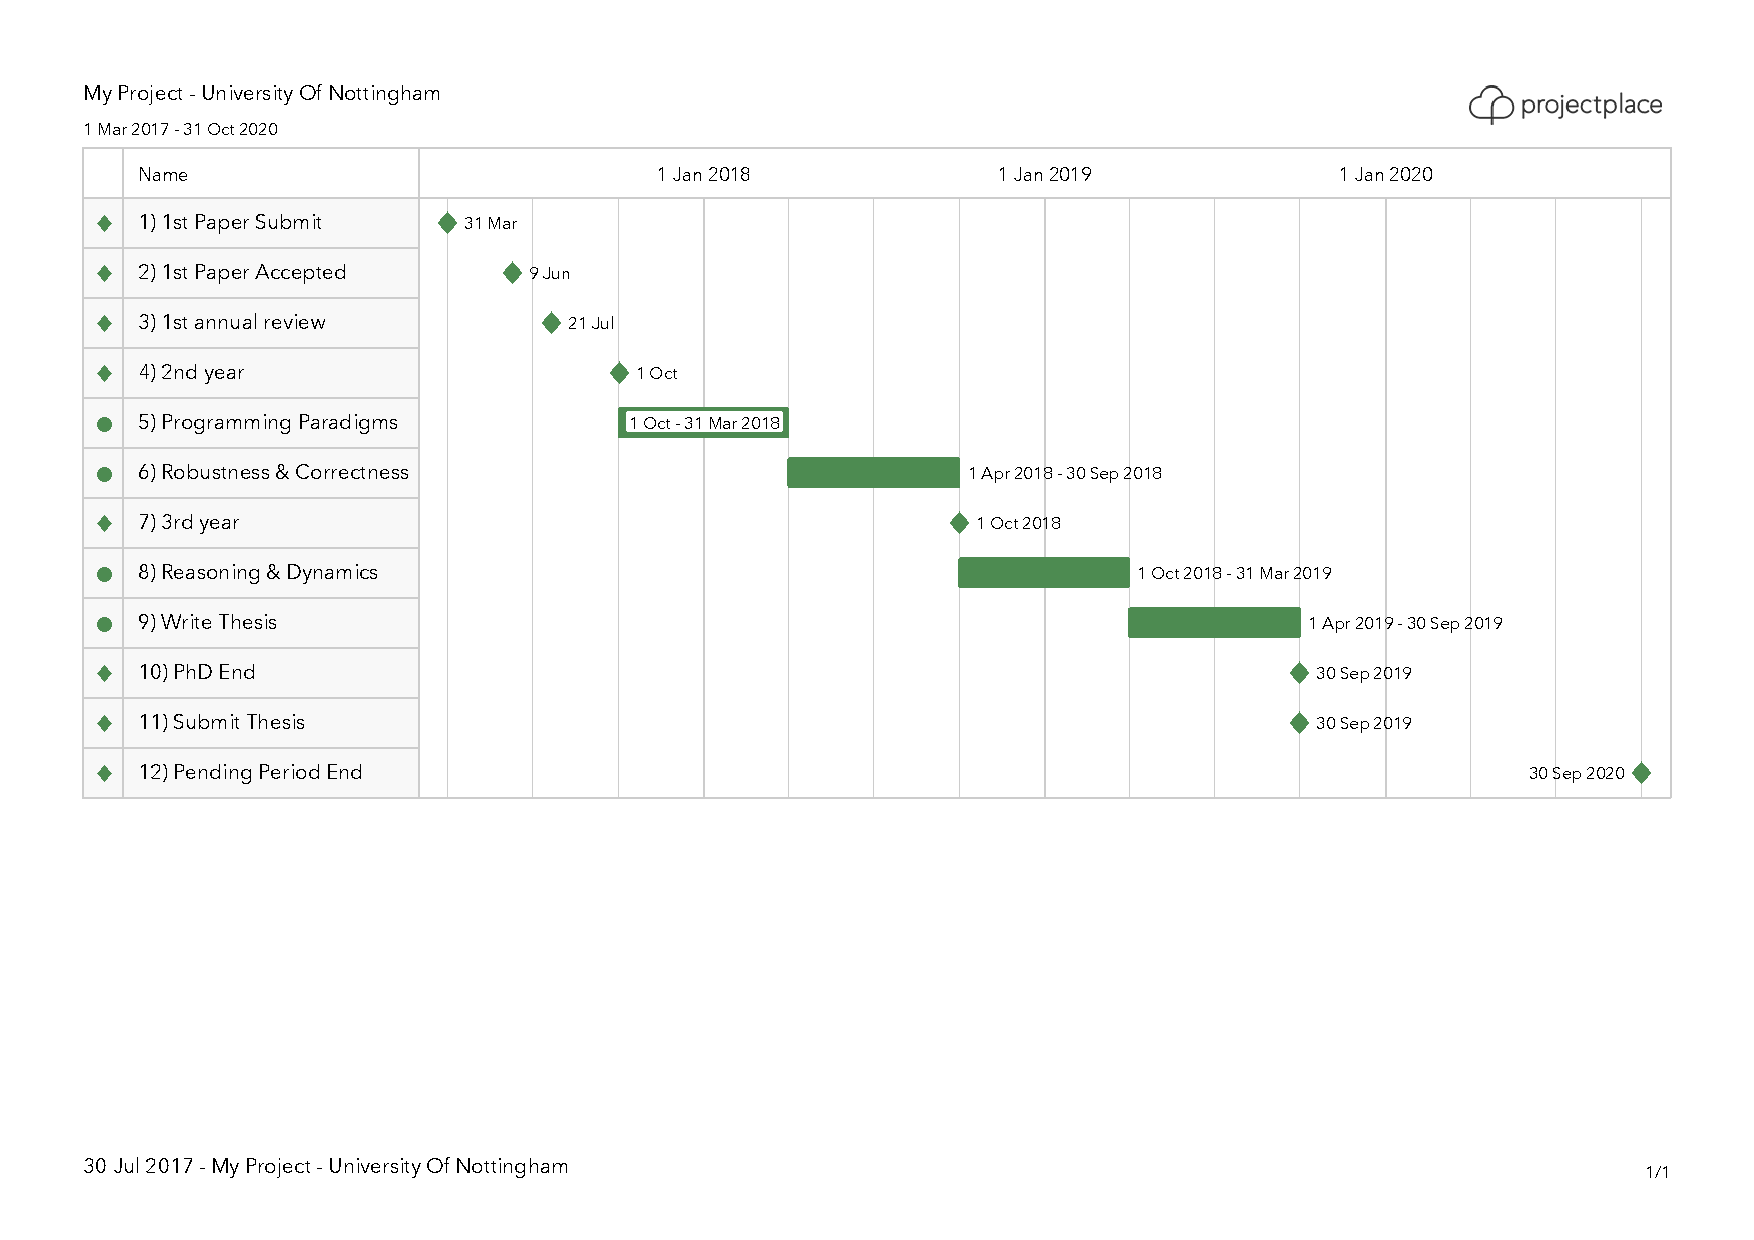
\includepdf[pages=-]{./charts/gantt.pdf}
%\end{landscape}

\begin{landscape}
\begin{figure}
	\centering
	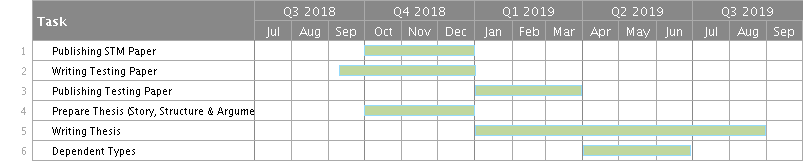
\includegraphics[width=1.5\textwidth, angle=0]{./fig/projectplan_3rd_year.png}
	\caption{Project Plan 3rd Year}
\end{figure}
\end{landscape}